\documentclass[9pt, aspectratio=169]{beamer}

% --- Custom Fonts and Engine Check ---
\usepackage{fontspec}
\usepackage{microtype}
\usepackage{amsmath, amsfonts, amssymb, amsthm}
\usepackage{mathtools}
\usepackage{physics}
\usepackage{siunitx}
\usepackage{tikz}
\usepackage{appendixnumberbeamer}
\usepackage{graphicx}
\usepackage{booktabs}
\usepackage{caption}
\usepackage{subcaption}
\usepackage{multirow}
\usepackage{multimedia}
\newwrite\notesfile
\immediate\openout\notesfile=\jobname.notes
\renewcommand{\note}[1]{%
  \immediate\write\notesfile{\thepage: \detokenize{#1}}%
}

\sisetup{locale = FR, separate-uncertainty = true}

% --- Figures Search Path ---
\graphicspath{
  {assets/}
  {/Users/emericmellet/Desktop/Emeric/School/UPS/M1 SGM/Stage/Repo/report/figures/}
  {/Users/emericmellet/Desktop/Emeric/School/UPS/M1 SGM/Stage/Repo/report/figures/slides/}
}

% --- Bibliography ---
\usepackage[backend=biber, style=numeric, sorting=none, defernumbers=true]{biblatex}
\addbibresource{bib/references.bib}

\DeclareBibliographyCategory{keyrefs}
\addtocategory{keyrefs}{%
  anderson1958,%
  derrida1984lyapounov,%
  tanguy2004weak,%
  beltukov2018propagative%
}

\defbibenvironment{bulletbib}
  {\list
     {\usebeamertemplate{itemize item}}
     {\setlength{\leftmargin}{2em}%
      \setlength{\itemindent}{0pt}%
      \setlength{\itemsep}{\bibitemsep}%
      \setlength{\parsep}{\bibparsep}}}
  {\endlist}
  {\item}

% --- Custom Theme Colors (Matching Figure Theme) ---
\definecolor{figureblue}{HTML}{1F77B4}   % Professional Blue (Disordered/TMM/Dispersion)
\definecolor{figureteal}{HTML}{00897B}   % Professional Dark Teal (DOS)
\definecolor{figurered}{HTML}{D62728}    % Professional Red (Theory/Matsuda/Optic)
\definecolor{figuregreen}{HTML}{2CA02C}  % Professional Green (Ballistic)
\definecolor{charcoal}{HTML}{2C3E50}     % Dark Charcoal for text
\definecolor{lightbg}{HTML}{F8F9FA}      % Light background for header/footer

% --- Beamer General Style Settings ---
\usecolortheme{default}
\usefonttheme{professionalfonts}

% Main colors
\setbeamercolor{background canvas}{bg=white}
\setbeamercolor{normal text}{fg=charcoal}
\setbeamercolor{structure}{fg=figureblue}
\setbeamercolor{alerted text}{fg=figurered}
\setbeamercolor{example text}{fg=figuregreen}

% Custom Block Styles
\setbeamercolor{block title}{fg=figureblue, bg=figureblue!12}
\setbeamercolor{block body}{fg=charcoal, bg=figureblue!4}
\setbeamercolor{block title alerted}{fg=figurered, bg=figurered!12}
\setbeamercolor{block body alerted}{fg=charcoal, bg=figurered!4}
\setbeamercolor{block title example}{fg=figuregreen, bg=figuregreen!12}
\setbeamercolor{block body example}{fg=charcoal, bg=figuregreen!4}

\setbeamertemplate{blocks}[rounded][shadow=false]

% Navigation Symbols
\setbeamertemplate{navigation symbols}{}

% --- Fallback University and Lab Logos ---
\newcommand{\universitylogo}[1][0.5cm]{%
  \IfFileExists{logo-ups.pdf}{%
    
\includegraphics[height=#1,keepaspectratio]{logo-ups.pdf}%
  }{%
    
\begin{tikzpicture}[baseline=(char.base)]
      \node[draw=figureblue!60, fill=figureblue!5, rounded corners=2pt, inner sep=3pt] (char) {\tiny\bfseries\sffamily\color{figureblue}UPSaclay};
    \end{tikzpicture}%
  }%
}

\newcommand{\lablogo}[1][0.5cm]{%
  \IfFileExists{lms-logo.pdf}{%
    
\includegraphics[height=#1,keepaspectratio]{lms-logo.pdf}%
  }{%
    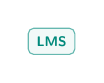
\begin{tikzpicture}[baseline=(char.base)]
      \node[draw=figureteal!60, fill=figureteal!5, rounded corners=2pt, inner sep=3pt] (char) {\tiny\bfseries\sffamily\color{figureteal}LMS};
    \end{tikzpicture}%
  }%
}

\setbeamertemplate{headline}{%
  \begin{beamercolorbox}[wd=\paperwidth,ht=7ex,dp=0pt,leftskip=2ex,rightskip=2ex]{headline}%
    \usebeamerfont{headline}%
    \parbox[b][7ex][c]{0.65\paperwidth}{%
      \bfseries\color{figureblue}%
      \insertsection%
      \ifx\insertsubsection\empty\else\ \ $\rightarrow$\ \ \normalfont\color{charcoal!80}\insertsubsection\fi%
    }%
    \hfill%
    \parbox[b][7ex][c]{0.28\paperwidth}{%
      \raggedleft%
      \universitylogo%
      \hspace{0.5em}%
      \lablogo%
    }%
  \end{beamercolorbox}%
  \color{figureblue!30}\hrule height 0.5pt%
}

% --- Custom Footer (Footline) ---
\setbeamertemplate{footline}{%
  \color{figureblue!20}\hrule height 0.5pt%
  \begin{beamercolorbox}[wd=\paperwidth,ht=3ex,dp=1.5ex,leftskip=2ex,rightskip=2ex]{footline}%
    \usebeamerfont{footline}%
    \color{charcoal!70}%
    \insertshorttitle%
    \hfill%
    \makebox[0pt][c]{Emeric Mellet}%
    \hfill%
    \insertframenumber\,/\,\inserttotalframenumber%
  \end{beamercolorbox}%
}

% --- Custom Frametitle ---
\setbeamertemplate{frametitle}{%
  \vspace*{1ex}%
  {\bfseries\large\color{figureblue}\insertframetitle}%
  \par\vspace*{0.5ex}%
}

% --- Custom Source Citation Command ---
\newcommand{\source}[1]{%
  \begin{tikzpicture}[remember picture,overlay]
    \node[anchor=south west, xshift=2ex, yshift=4.5ex] at (current page.south west) {%
      \usebeamerfont{footnote}\scriptsize\color{charcoal!60}\textit{Source : #1}%
    };
  \end{tikzpicture}%
}

% --- Itemize Styles ---
\setbeamertemplate{itemize items}[circle]
\setbeamercolor{itemize item}{fg=figureblue}
\setbeamercolor{itemize subitem}{fg=figureteal}

% --- Metadata ---
\title[Soutenance de Stage M1 SGM]{Propagation d'ondes dans les chaînes harmoniques 1D désordonnées}
\subtitle{Bilan scientifique et pédagogique de stage de recherche}
\author{Emeric Mellet}
\institute{Université Paris-Saclay}
\newcommand{\hostinstitute}[1]{\def\inserthostinstitute{#1}}
\hostinstitute{Laboratoire de Mécanique des Solides (LMS), École Polytechnique}
\date{8 Juillet 2026}

% ==========================================
%                  SLIDES
% ==========================================
\begin{document}

% --- Slide 1: Plain ---
\begin{frame}[plain]
  \begin{tikzpicture}[remember picture, overlay]
    % Background styling
    % \fill[figureblue!5] (current page.south west) rectangle (current page.north east);
    % \fill[figureblue, opacity=0.08] (current page.south west) rectangle (current page.north east);
    % \fill[figureblue, opacity=0.08] (current page.south west) -- (current page.north east) -- (current page.south east) -- cycle;
    \node[anchor=center, inner sep=0pt, outer sep=0pt] at (current page.center) {\includegraphics[width=\paperwidth,height=\paperheight]{bg_title.pdf}};

    % Logos at top
    \node[anchor=north west, xshift=0.8cm, yshift=-0.6cm] at (current page.north west) {\universitylogo[1.1cm]};
    \node[anchor=north east, xshift=-0.8cm, yshift=-0.6cm] at (current page.north east) {\lablogo[1.1cm]};

    % Title Info
    \node[anchor=center, align=center, text width=0.72\paperwidth, yshift=-0.2cm] at (current page.center) {
    {\Large\bfseries\color{figureblue}\inserttitle}\\[0.3cm]
    {\large\color{charcoal}\insertsubtitle}\\[0.8cm]
    \textbf{\color{charcoal}\insertauthor}\\[0.2cm]
    {\small\color{charcoal!85}Réferent : Jérôme Creuze}\\[0.2cm]
    {\small\color{charcoal!70}\insertinstitute}\\[0.3cm]
    {\small\color{charcoal!85}Encadrante : Anne Tanguy}\\[0.2cm]
    {\small\color{charcoal!70}\inserthostinstitute}\\[0.5cm]
    {\small\color{charcoal!85}\insertdate}
    };
  \end{tikzpicture}

  \note{Bonjour à tous. Merci d'être venus pour ma soutenance de stage. J'ai effectué mon travail de recherche au LMS à l'École Polytechnique, sous la direction d'Anne Tanguy. Mon sujet porte sur la propagation d'ondes dans les chaînes 1D désordonnées. C'est un travail à la fois théorique et numérique.}
\end{frame}

% --- Slide 2: Table des Matières ---
\begin{frame}[plain]
  \frametitle{Table des Matières}
  \vspace*{2ex}
  \begin{columns}[t]
    \begin{column}{0.48\textwidth}
      \begin{block}{Partie I : Étude Scientifique}
        \begin{itemize}
          \item Contexte et phénomènes de transport
          \item Modèles analytiques (Modale, Matriciel, Riccati)
          \item Simulations dynamiques (Verlet)
          \item Résultats et comparaison des approches
        \end{itemize}
      \end{block}
    \end{column}
    \begin{column}{0.48\textwidth}
      \begin{block}{Partie II : Bilan Professionnel et Perspectives}
        \begin{itemize}
          \item Immersion au sein du Laboratoire (LMS)
          \item Bilan des compétences et outils (Python, \LaTeX, Git)
          \item Choix académiques et transition vers le M2 MAMI
          \item Conclusion générale et perspectives scientifiques
        \end{itemize}
      \end{block}
    \end{column}
  \end{columns}

  \note{Voici le plan de ma présentation. Nous commencerons par la partie scientifique. Je rappellerai les régimes de transport ondulatoire, puis je décrirai la modélisation dynamique par l'intégration d'un paquet d'ondes. Nous verrons ensuite comment l'analyse modale de la matrice dynamique se compare au formalisme matriciel à fréquence fixe avec les matrices de transfert et la carte de Riccati. Enfin, nous confronterons les résultats de ces trois approches avant de passer au bilan professionnel de mon stage.}
\end{frame}

% --- Section 1: Contexte et Introduction ---
\section{Contexte et Introduction}
\subsection{Contexte physique}

% --- Slide 3: Origine du Projet : Des simulations 3D à la chaîne 1D ---
\begin{frame}{Origine du Projet : Des simulations 3D à la chaîne 1D}
  \begin{columns}[c]
    \begin{column}{0.55\textwidth}
      \textbf{Simulations 3D préalables} :
      \begin{itemize}
        \item Modélisation d'un solide amorphe.
        \item Propagation d'ondes élastiques \& transition de localisation des phonons.
      \end{itemize}

      \vspace*{1.5ex}
      \begin{block}{Nécessité de l'étude 1D}
        Incertitude sur l'origine du confinement :
        \begin{itemize}
          \item Effet des \alert{non-linéarités} des interactions ?
          \item Effet pur du \alert{désordre} (masses, raideurs) ?
        \end{itemize}
        $\Rightarrow$ Besoin d'un système linéaire 1D pour séparer ces deux contributions physiques.
      \end{block}
    \end{column}
    \begin{column}{0.42\textwidth}
      \centering
      \scriptsize

      \textbf{Faible} (Longitudinal, $A = 0{,}1\text{ eV/\AA}$) \\
      \vspace*{0.2ex}
      \IfFileExists{CuZr-Low_snapshot.png}{%
        \href{run:assets/CuZr-Low.mp4?autostart\string&noprogress}{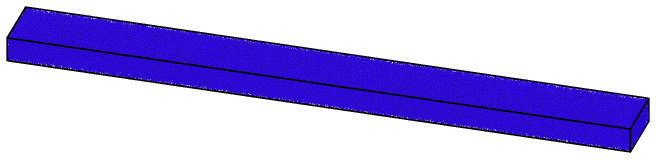
\includegraphics[width=0.70\textwidth]{CuZr-Low_snapshot.png}}%
      }{%
        
\begin{tikzpicture}[draw=figureblue!50, fill=figureblue!5, thick]
          \draw[rounded corners=4pt, fill=lightbg] (0,0) rectangle (2.5,0.6);
          \node[color=charcoal] at (1.25,0.3) {\tiny [CuZr-Low]};
        \end{tikzpicture}
      }%
      \vspace*{0.8ex}

      \textbf{Moyen} (Longitudinal, $A = 1\text{ eV/\AA}$) \\
      \vspace*{0.2ex}
      \IfFileExists{CuZr-Med_snapshot.png}{%
        \href{run:assets/CuZr-Med.mp4?autostart\string&noprogress}{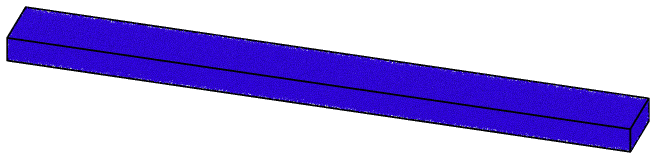
\includegraphics[width=0.70\textwidth]{CuZr-Med_snapshot.png}}%
      }{%
        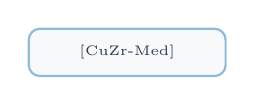
\begin{tikzpicture}[draw=figureblue!50, fill=figureblue!5, thick]
          \draw[rounded corners=4pt, fill=lightbg] (0,0) rectangle (2.5,0.6);
          \node[color=charcoal] at (1.25,0.3) {\tiny [CuZr-Med]};
        \end{tikzpicture}
      }%
      \vspace*{0.8ex}

      \textbf{Fort} (Transversal, $A = 1\text{ eV/\AA}$) \\
      \vspace*{0.2ex}
      \IfFileExists{CuZr-Hi_snapshot.png}{%
        \href{run:assets/CuZr-Hi.mp4?autostart\string&noprogress}{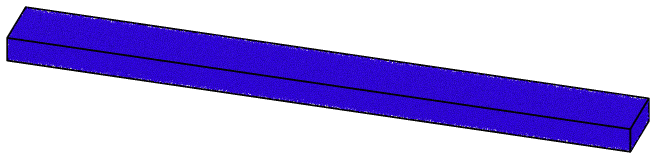
\includegraphics[width=0.70\textwidth]{CuZr-Hi_snapshot.png}}%
      }{%
        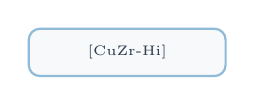
\begin{tikzpicture}[draw=figureblue!50, fill=figureblue!5, thick]
          \draw[rounded corners=4pt, fill=lightbg] (0,0) rectangle (2.5,0.6);
          \node[color=charcoal] at (1.25,0.3) {\tiny [CuZr-Hi]};
        \end{tikzpicture}
      }%

      \vspace*{0.8ex}
      \captionof{figure}{Ondes dans CuZr amorphe ($\nu = 0{,}5\text{ THz}$) par R. Alvarez et A. Tanguy.}
    \end{column}
  \end{columns}

  \note{Avant d'aborder les modèles analytiques, il est important de comprendre la genèse de ce projet. Pour cela, nous sommes partis de simulations 3D d'un matériau désordonné (le CuZr amorphe) réalisées par mon encadrante, Anne Tanguy. Les animations à droite illustrent la propagation d'un paquet d'ondes sous trois conditions : un désordre faible et moyen pour des ondes longitudinales, et un désordre fort pour des ondes transverses. On constate que la propagation est fortement affectée par la nature de l'onde et le niveau de désordre. Ces travaux laissaient une incertitude : quelle est la part due aux non-linéarités et quelle est celle due uniquement au désordre de masse ou de raideur ? C'est pour lever ce doute et isoler le désordre harmonique linéaire que nous étudions un modèle 1D.}
\end{frame}

\subsection{Phénomènes de transport vibratoire}
% --- Slide 4: Introduction : Phénomènes de transport vibratoire ---
\begin{frame}{Introduction : Phénomènes de transport vibratoire}
  \begin{itemize}
    \item \textbf{Milieu périodique (Cristal parfait)} : Transport balistique ($\sigma^2(t) \propto t^2$, sans atténuation).
    \item \textbf{Milieu stochastiquement désordonné} : Brisure de symétrie de translation.
          \begin{itemize}
            \item En dimension $d \geq 3$ : transition balistique $\to$ diffusif $\to$ localisé.
            \item \textbf{Choix du 1D} : existence de solutions analytiques exactes (Derrida-Gardner, Matsuda-Ishii), intraitables en 2D/3D.
            \item \textbf{Propriété} : tous les états y sont localisés (Abrahams et al., 1979 \cite{abrahams1979scaling}).
          \end{itemize}
  \end{itemize}
  \vspace*{1.5ex}
  \begin{block}{Objectif du Stage}
    Caractériser la localisation des ondes dans un système unidimensionnel désordonné acoustique par comparaison de quatre approches numériques complémentaires.
  \end{block}

  \note{Dans un cristal parfait, la propagation est balistique. Dès qu'on introduit du désordre, la symétrie de translation est brisée. Pour étudier ce problème, nous choisissons un modèle 1D. Ce n'est pas uniquement parce que tous les états y sont localisés (ce qui est une propriété physique intéressante, un « accident heureux »), mais surtout parce que la dimension 1 offre des modèles analytiques exacts (comme Derrida-Gardner ou Matsuda-Ishii) qui sont mathématiquement insolubles en 2D et 3D. L'objectif de mon stage est de caractériser cette localisation par quatre méthodes numériques et de les confronter à ces théories exactes.}
\end{frame}

% --- Slide 5: Visualisation Dynamique : Ordonné vs Localisé ---
\begin{frame}{Visualisation Dynamique : Ordonné vs Localisé}
  \begin{columns}[c]
    \begin{column}{0.46\textwidth}
      \small
      \textbf{Réseau 1D}
      \begin{itemize}
        \item \textbf{Masses et raideurs} : Valeurs locales $M_j, K_j$ (désordre).
        \item \textbf{Normalisation} : $m_0 = 1, K_0 = 1, a = 1$.
      \end{itemize}
      \vspace*{1ex}
      \textbf{Excitation (Paquet d'Ondes)}
      \begin{itemize}
        \item Gaussienne modulée au centre $j_c$ : \\
              {\scriptsize $u_{j_c}(t) \propto e^{-2\sigma (t-t_0)^2} \sin(\omega_{\text{ext}} (t-t_0))$}
        \item Pulsation porteuse : $\omega_{\text{ext}} = 1.1$
      \end{itemize}
      \vspace*{1ex}
      \textbf{Propagation du Paquet}
      \begin{itemize}
        \item \textbf{Ordonné} : Séparation symétrique (propagation balistique).
        \item \textbf{Désordonné} : Piégeage (localisation d'Anderson).
      \end{itemize}
      \vspace*{1ex}
      {\scriptsize\color{charcoal!70}\textit{N.B.} : $\omega_{\text{ext}}$ choisie proche de la limite de Brillouin ($\omega_{\max}^0 = 2$) $\Rightarrow$ effets de réseau discrets visibles.}
    \end{column}
    \begin{column}{0.5\textwidth}
      \centering
      \IfFileExists{wave_propagation.mp4}{%
        \href{run:assets/wave_propagation.mp4?autostart}{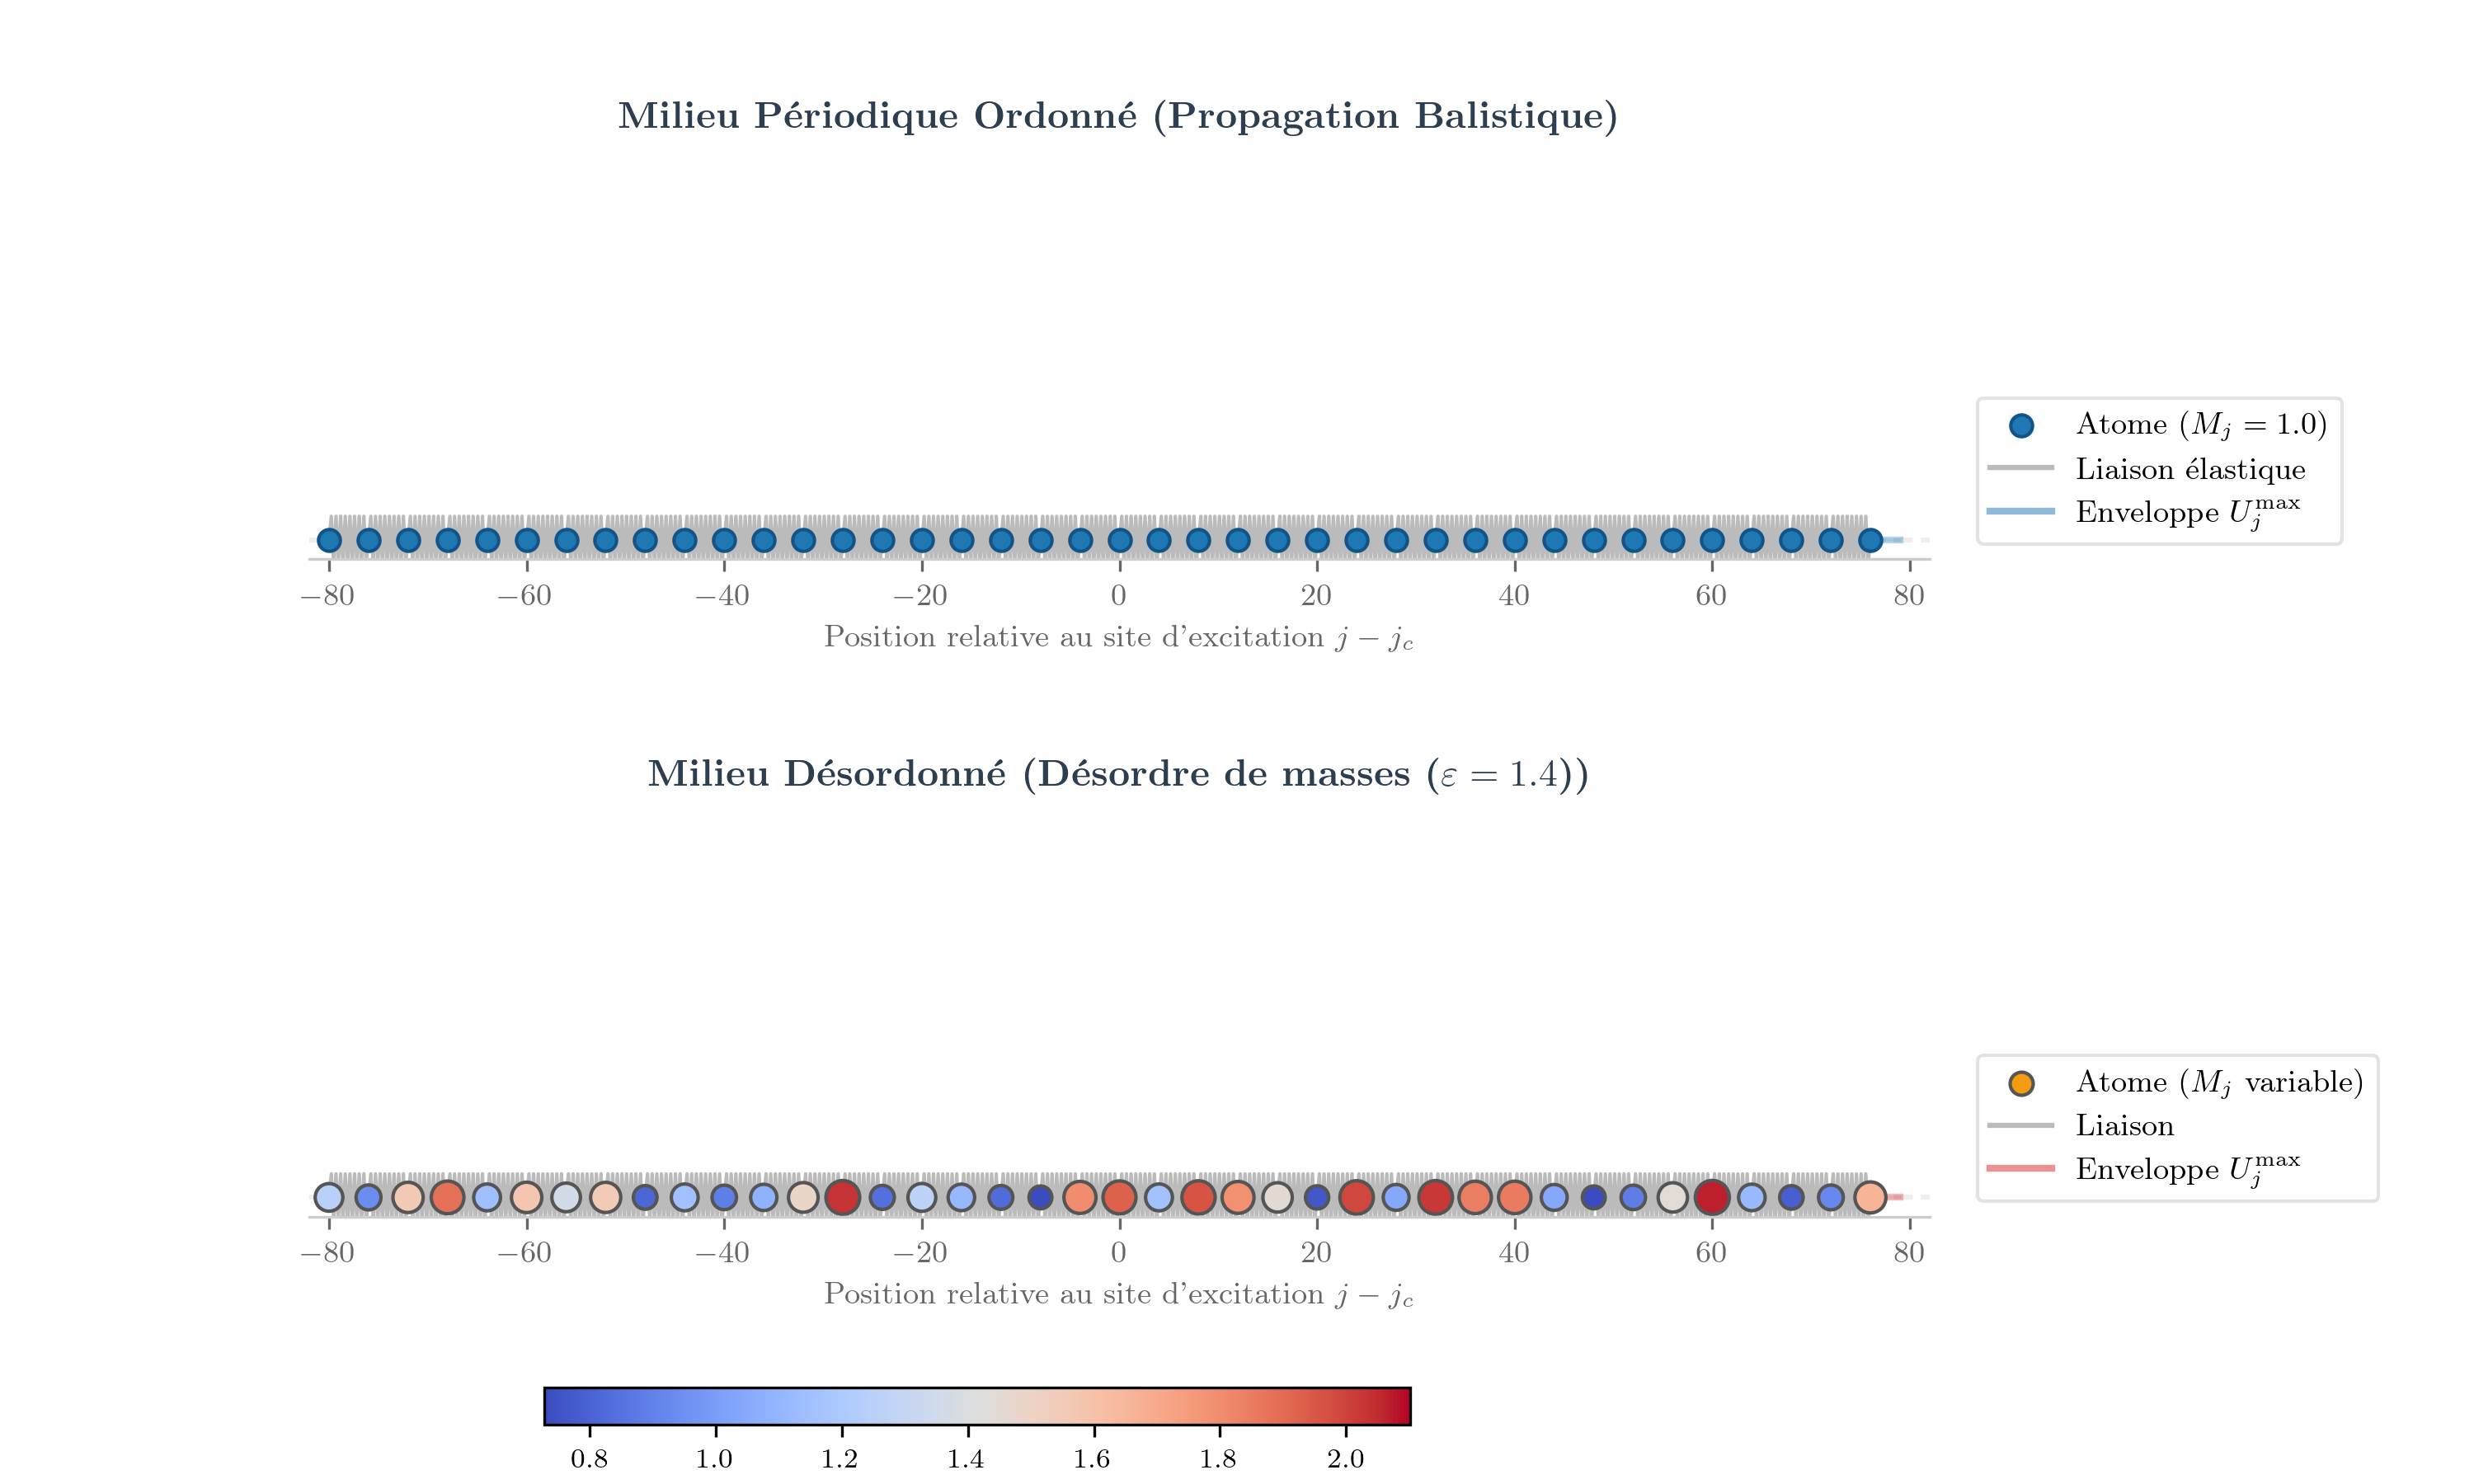
\includegraphics[width=\textwidth]{wave_propagation_snapshot.png}}%
      }{%
        \IfFileExists{wave_propagation_snapshot.png}{%
          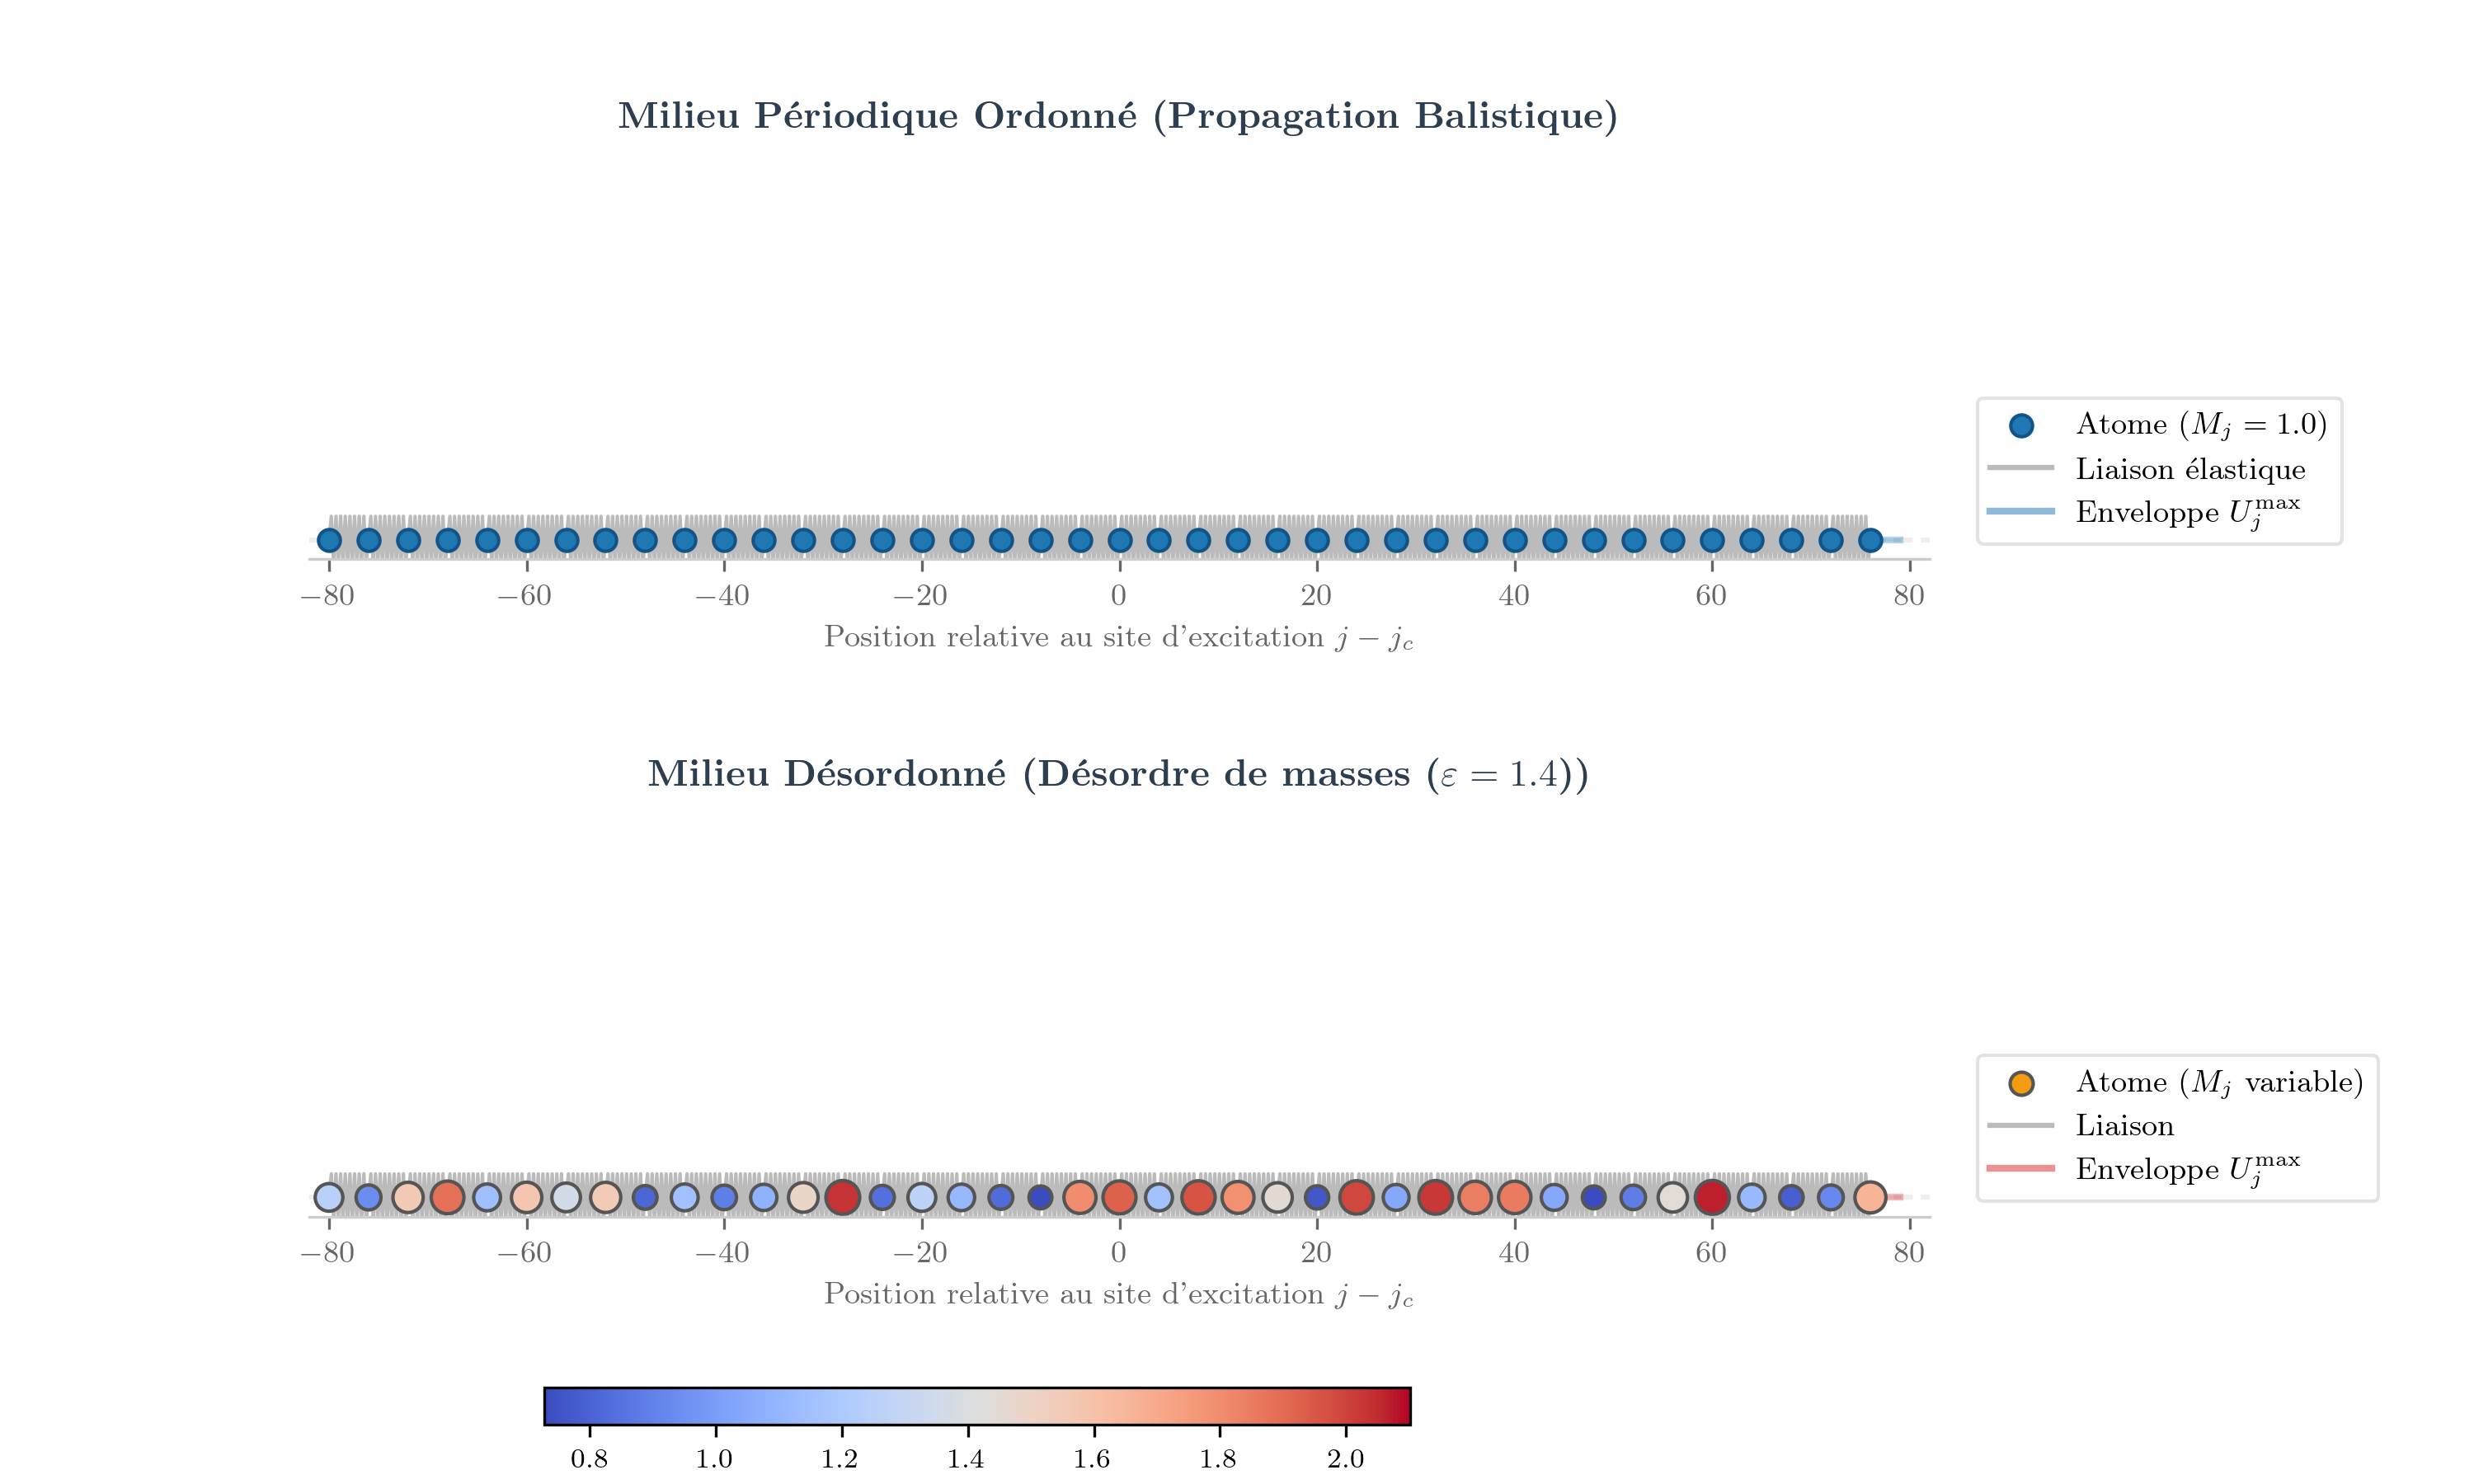
\includegraphics[width=\textwidth]{wave_propagation_snapshot.png}%
        }{%
          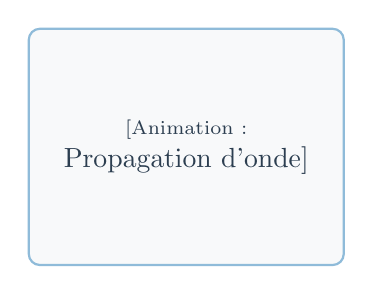
\begin{tikzpicture}[draw=figureblue!50, fill=figureblue!5, thick]
            \draw[rounded corners=4pt, fill=lightbg] (0,0) rectangle (4,3);
            \node[align=center, color=charcoal] at (2,1.5) {\scriptsize [Animation :\\ Propagation d'onde]};
          \end{tikzpicture}
        }%
      }%
      \captionof{figure}{Simulation dynamique : ordonné (haut) vs désordonné (bas)}
    \end{column}
  \end{columns}


  \note{Voici la simulation dynamique en 1D. En haut, dans un réseau parfaitement ordonné, l'onde se propage librement à vitesse constante. En bas, en présence de désordre, on observe un piégeage rapide de l'énergie : le paquet d'ondes s'arrête et reste confiné au centre. C'est l'illustration visuelle directe de la localisation d'Anderson.}
\end{frame}

% --- Slide 6: Les trois régimes de transport ondulatoire ---
\begin{frame}{Les trois régimes de transport ondulatoire}
  \begin{columns}[c]
    \begin{column}{0.5\textwidth}
      \begin{itemize}
        \item \textbf{\color{figuregreen}Régime Balistique} : Ondes planes progressives, sans déformation.
        \item \textbf{\color{figureblue}Régime Diffusif} : Étalement stochastique (marche aléatoire).
        \item \textbf{\color{figurered}Régime Localisé} : Décroissance exponentielle, confinement.
      \end{itemize}
      \vspace*{2ex}
      \begin{block}{Variance Spatiale}
        $\sigma^2(t) = \sum_{n} (n - n_0)^2 |u_n(t)|^2$
      \end{block}
    \end{column}
    \begin{column}{0.48\textwidth}
      \centering
      \IfFileExists{/Users/emericmellet/Desktop/Emeric/School/UPS/M1 SGM/Stage/Repo/report/figures/01_historical_context.pdf}{%
        \includegraphics[width=\textwidth,keepaspectratio]{01_historical_context.pdf}%
      }{%
        \begin{tikzpicture}[draw=figureblue!50, fill=figureblue!5, thick]
          \draw[rounded corners=4pt, fill=lightbg] (0,0) rectangle (5,3.5);
          \node[align=center, color=charcoal] at (2.5,1.75) {
          \begin{tikzpicture}[scale=0.5]
            \draw[->] (0,0) -- (4,0);
            \draw[->] (0,0) -- (0,3);
            \draw[color=figurered, thick] (0,0) to[out=30,in=150] (2,2) to[out=-30,in=180] (4,0.5);
          \end{tikzpicture}\\
          [0.2cm]\tiny [Figure: 01\_historical\_context.pdf]
          };
        \end{tikzpicture}
      }%
      \captionof{figure}{Propagation de l'enveloppe temporelle dans un système $d\geq2$}
    \end{column}
  \end{columns}
  \source{Hu et al. (2008) \cite{hu2008localization}}





  \note{Pour quantifier cela, on suit l'étalement de l'onde par sa variance. Ce graphique montre les trois régimes types : en vert, le régime balistique sans obstacle ; en bleu, le régime diffusif comparable à une marche aléatoire ; et en rouge, la localisation forte où l'onde cesse de s'étaler après un certain temps, formant une enveloppe stationnaire et figée.}
\end{frame}


% --- Section 2: Modèles Analytiques ---
\section{Modèles Analytiques}
\subsection{Théorie des modèles analytiques}

% --- Slide 7: Analyse Modale : Équation Matricielle et Valeurs Propres ---
\begin{frame}{Analyse Modale : Équation Matricielle et Valeurs Propres}
  Équation dynamique ($M$ et $K$ symétriques) :
  \begin{equation}
    M \ddot{u} + K u = 0
  \end{equation}
  Solutions harmoniques $u(t) = \phi e^{i\omega t} \Rightarrow$ Problème généralisé :
  \begin{equation}
    K \phi = \omega^2 M \phi
  \end{equation}
  Problème standard symétrique ($\tilde{\phi} = M^{1/2}\phi \Rightarrow \sum_i \tilde{\phi}_i^2 = 1$) :
  \begin{equation}
    \tilde{K} \tilde{\phi} = \omega^2 \tilde{\phi} \qquad \text{avec} \quad \tilde{K} = M^{-1/2} K M^{-1/2}
  \end{equation}

  \begin{block}{Taux de Participation ($PR$)}
    Proportion de sites actifs ($\sum_i \tilde{\phi}_i^2 = 1$) :
    \begin{equation}
      P_R = \frac{1}{N\sum_{i=1}^N \tilde{\phi}_{i}^4} \quad \Longrightarrow \quad
      \begin{cases}
        P_R \to 1   & \text{(Mode étendu)}   \\
        P_R \to 1/N & \text{(Mode localisé)}
      \end{cases}
    \end{equation}
  \end{block}

  \note{L'analyse modale repose sur l'équation dynamique sous forme matricielle $M \ddot{u} + K u = 0$. En cherchant des solutions harmoniques, on obtient le problème aux valeurs propres généralisé $K \phi = \omega^2 M \phi$. Bien que la matrice de raideur $K$ soit symétrique par définition, on se ramène à un problème aux valeurs propres standard symétrique $\tilde{K} \tilde{\phi} = \omega^2 \tilde{\phi}$ (où $\tilde{K} = M^{-1/2} K M^{-1/2}$ est symétrique) afin d'obtenir des modes propres orthonormalisés au sens usuel. Enfin, le taux de participation (PR) quantifie la proportion de sites actifs pour chaque mode, variant entre $1/N$ et $1$.}
\end{frame}

% --- Slide 8: Méthode des Matrices de Transfert \& Carte de Riccati ---
\begin{frame}{Méthode des Matrices de Transfert \& Carte de Riccati}
  Récurrence spatiale à fréquence fixe $\omega$ :
  \begin{equation}
    \begin{pmatrix} u_{n+1} \\ u_n \end{pmatrix} = T_n \begin{pmatrix} u_n \\ u_{n-1} \end{pmatrix} \quad \text{avec} \quad T_n = \begin{pmatrix} \frac{K_n + K_{n-1} - m_n\omega^2}{K_n} & -\frac{K_{n-1}}{K_n} \\ 1 & 0 \end{pmatrix}
  \end{equation}
  Longueur de localisation $\xi$ via l'exposant de Lyapunov $\gamma$ :
  \begin{equation}
    \gamma = \lim_{N \to \infty} \frac{1}{N} \ln \big\| T_N T_{N-1} \dots T_1 \big\| = \xi^{-1}
  \end{equation}

  \begin{alertblock}{Stabilisation par Carte de Riccati}
    Évite la divergence numérique du produit de matrices. Variable $R_n = u_{n+1} / u_n$ :
    \begin{equation}
      R_n = 2 - \frac{m_n\omega^2}{K} - \frac{1}{R_{n-1}} \qquad (\text{raideurs uniformes } K_n = K)
    \end{equation}
  \end{alertblock}



  \note{La méthode des matrices de transfert permet de calculer la propagation à une fréquence fixe de proche en proche. En multipliant ces matrices, on extrait l'exposant de Lyapunov et donc la longueur de localisation. Pour éviter les divergences numériques de ce produit, on utilise la carte de Riccati en étudiant le rapport des déplacements consécutifs. Cela stabilise la récurrence et sert de base aux modèles analytiques.}
\end{frame}


% --- Slide 9: Comparaison des Modèles Analytiques ---
\begin{frame}{Comparaison des Modèles Analytiques}
  \begin{center}
    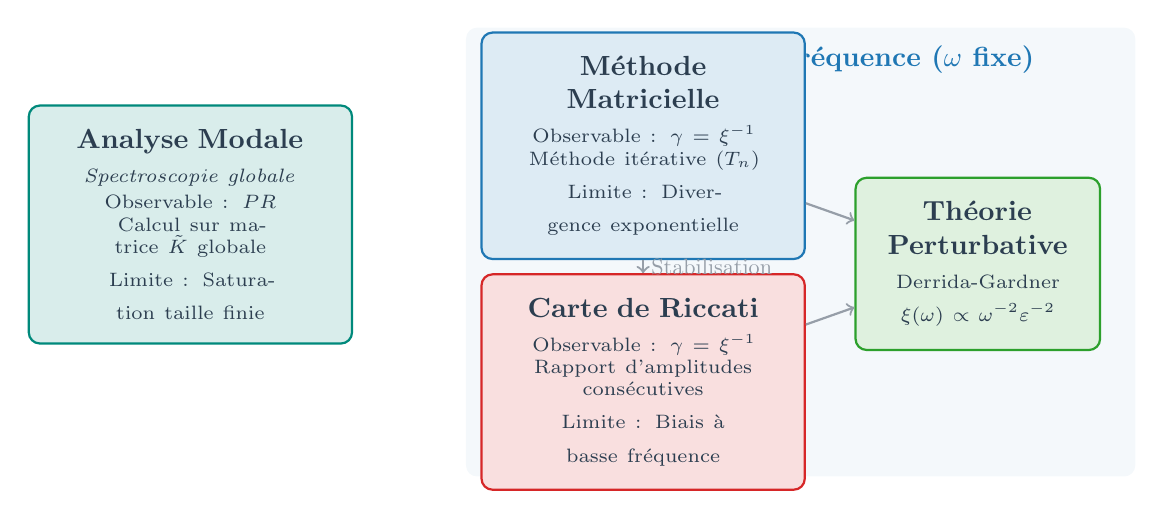
\begin{tikzpicture}
      % Dessin d'un tableau/diagramme de type Euler/Karnaugh
      % On définit les styles
      \tikzstyle{box} = [draw, rounded corners, thick, text centered, inner sep=2ex, text=charcoal]
      \tikzstyle{modal} = [box, fill=figureteal!15, draw=figureteal, text width=3.5cm]
      \tikzstyle{tmm} = [box, fill=figureblue!15, draw=figureblue, text width=3.5cm]
      \tikzstyle{riccati} = [box, fill=figurered!15, draw=figurered, text width=3.5cm]

      % Background encompassing TMM & Riccati
      \fill[figureblue!5, rounded corners] (3.5, -3.2) rectangle (12, 2.5);
      \node[color=figureblue, font=\bfseries] at (7.75, 2.1) {Formalisme de Fréquence ($\omega$ fixe)};

      % Modal Box
      \node[modal] (mod) at (0, 0) {
        \textbf{Analyse Modale}\\[1ex]
        \scriptsize
        \textit{Spectroscopie globale}\\[0.5ex]
        Observable : $PR$\\
        Calcul sur matrice $\tilde{K}$ globale\\
        Limite : Saturation taille finie
      };

      % TMM Box
      \node[tmm] (tmm) at (5.75, 1) {
        \textbf{Méthode Matricielle}\\[1ex]
        \scriptsize
        Observable : $\gamma = \xi^{-1}$\\
        Méthode itérative ($T_n$)\\
        Limite : Divergence exponentielle
      };

      % Riccati Box
      \node[riccati] (ric) at (5.75, -2) {
        \textbf{Carte de Riccati}\\[1ex]
        \scriptsize
        Observable : $\gamma = \xi^{-1}$\\
        Rapport d'amplitudes consécutives\\
        Limite : Biais à basse fréquence
      };

      % Arrows
      \draw[->, thick, color=charcoal!50] (tmm) -- node[right, scale=0.8] {Stabilisation} (ric);

      % Joint box
      \node[box, fill=figuregreen!15, draw=figuregreen, text width=2.5cm] (dyn) at (10, -0.5) {
        \textbf{Théorie \\ Perturbative}\\[1ex]
        \scriptsize
        Derrida-Gardner\\
        $\xi(\omega) \propto \omega^{-2} \varepsilon^{-2}$
      };
      \draw[->, thick, color=charcoal!50] (tmm) -- (dyn);
      \draw[->, thick, color=charcoal!50] (ric) -- (dyn);

    \end{tikzpicture}
  \end{center}

  \note{Avant de passer aux simulations temporelles, voici comment se situent ces modèles analytiques. À gauche, l'analyse modale donne une vision globale du spectre mais souffre de la taille finie. À droite, les méthodes à fréquence fixe : les matrices de transfert et la carte de Riccati. Elles calculent toutes deux la même observable : l'inverse de la longueur de localisation. Riccati dérive directement de la méthode matricielle pour stabiliser ses divergences numériques, et ces deux approches permettent de retrouver le comportement analytique perturbatif aux basses fréquences.}
\end{frame}
% --- Section 3: Simulations Dynamiques ---
\section{Simulations Dynamiques}
\subsection{Théorie des simulations dynamiques}

% --- Slide 10: Réseau 1D Masse-Ressort \& Schéma Symplectique ---
\begin{frame}{Réseau 1D Masse-Ressort \& Schéma Symplectique}
  Dynamique harmonique d'une chaîne 1D :
  \begin{equation}
    m_n \ddot{u}_n = K_n (u_{n+1} - u_n) - K_{n-1} (u_n - u_{n-1})
  \end{equation}
  Désordre ($r_n, s_n \in [-0.5,\, 0.5]$ variables uniformes indépendantes) :
  \begin{equation}
    m_n = m_0 (1 + \varepsilon_m \cdot r_n), \qquad K_n = K_0 (1 + \varepsilon_K \cdot s_n)
  \end{equation}
  \vspace*{-1.5ex}
  {\scriptsize\color{charcoal!70} ($r_n, s_n$ : fluctuations relatives locales de masse et de raideur ; $\varepsilon_m, \varepsilon_K$ : amplitudes de désordre)}
  \vspace*{1.5ex}

  \begin{block}{Simulation Temporelle : Leapfrog Verlet}
    Intégrateur symplectique ($\tau = \Delta t$), sans dérive d'énergie à long terme :
    \begin{align}
      v_n\left(t + \tfrac{\tau}{2}\right) & = v_n\left(t - \tfrac{\tau}{2}\right) + \tau \, a_n(t) + \mathcal{O}(\tau^3)                 \\
      u_n(t + \tau)                       & = u_n(t) + \tau \, v_n\left(t + \tfrac{\tau}{2}\right) + \mathcal{O}(\tau^3)                 \\
      a_n(t + \tau)                       & = \frac{1}{m_n} f_n\left(u_n(t + \tau), v_n\left(t + \tfrac{\tau}{2}\right), t + \tau\right)
    \end{align}
  \end{block}

  \note{Pour modéliser le réseau, on utilise une chaîne 1D de masses et de ressorts. Le désordre est introduit sur les masses ou sur les raideurs. Pour simuler la propagation dans le temps, on utilise l'algorithme de Leapfrog (Verlet). Ce schéma a la particularité d'être symplectique, c'est-à-dire qu'il conserve parfaitement l'énergie globale sans ajouter de frottement numérique artificiel, ce qui garantit la fiabilité des simulations à très long terme.}
\end{frame}
\subsection{Résultats: Analyse Modale}

% --- Slide 11: Spectroscopie Modale : Densité d'États \& Rapport de Participation ---
\begin{frame}{Spectroscopie Modale : Densité d'États \& Rapport de Participation}
  \begin{columns}[c]
    \begin{column}{0.58\textwidth}
      \centering
      \IfFileExists{/Users/emericmellet/Desktop/Emeric/School/UPS/M1 SGM/Stage/Repo/report/figures/slides/10_participation_ratio_slides.pdf}{%
        \includegraphics[width=\textwidth,height=0.70\textheight,keepaspectratio]{10_participation_ratio_slides.pdf}%
      }{%
        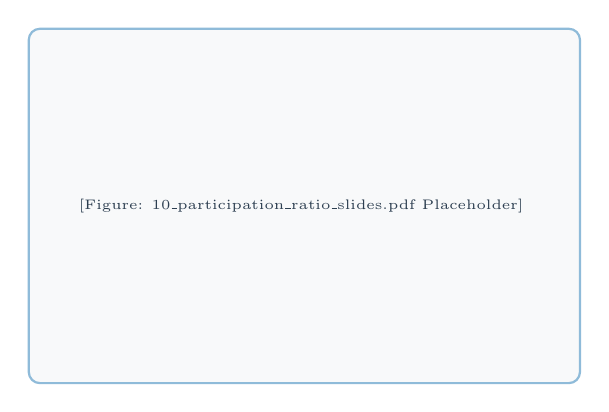
\begin{tikzpicture}[draw=figureblue!50, fill=figureblue!5, thick]
          \draw[rounded corners=4pt, fill=lightbg] (0,0) rectangle (7,4.5);
          \node[align=center, color=charcoal] at (3.5,2.25) {
            \tiny [Figure: 10\_participation\_ratio\_slides.pdf Placeholder]
          };
        \end{tikzpicture}
      }%
      \captionof{figure}{DOS et PR pour $\sigma_\varepsilon = 0.1,\, 0.7,\, 1.4$}
    \end{column}
    \begin{column}{0.38\textwidth}
      \footnotesize
      \begin{block}{Densité d'États $g(\omega)$}
        \begin{itemize}
          \item Érosion du gap à Bragg ($\omega = 2$).
          \item États de queue haute fréquence.
        \end{itemize}
      \end{block}

      \vspace*{1.5ex}
      \begin{block}{Taux de Participation $PR$}
        \begin{itemize}
          \item Modes $\omega > 2$ confinés.
          \item Saturation par taille finie à basse fréquence.
        \end{itemize}
      \end{block}
    \end{column}
  \end{columns}
  \source{Simulations LMS}



  \note{Sur ces graphiques, nous étudions les modes de vibration de la chaîne. Quand le désordre augmente, de nouveaux modes apparaissent à haute fréquence. Le graphique du bas montre que ces modes de haute fréquence sont très localisés, parfois confinés sur un seul atome. À basse fréquence, la taille finie de notre chaîne fermée sature le taux de participation car les modes tendent à dépasser la longueur de la chaîne.}
\end{frame}


\subsection{Résultats: Matriciel et Riccati}

% --- Slide 12: Validation de la Théorie Perturbative (Derrida \& Gardner) ---
\begin{frame}{Validation de la Théorie Perturbative (Derrida \& Gardner)}
  Développement en désordre faible ($\langle\epsilon_n^2\rangle \ll 1$) avec $\eta_n$ la fluctuation de phase complexe ($R_n = \mathrm{e}^{\mathrm{i}qa + \eta_n}$) :
  \begin{align}
    \gamma(q) & = \frac{\langle\epsilon_n^2\rangle}{8}\,\tan^2\!\left(\frac{qa}{2}\right) \qquad \xrightarrow{qa \ll 1} \qquad \gamma \approx \frac{\langle\epsilon_n^2\rangle\, q^2 a^2}{32} \\
    \eta_n    & = \left[ \eta_0 + \sum_{j=0}^{n-1} \frac{A_j(qa)}{\prod_{k=0}^{j} B_k(qa)} \right] \prod_{k=0}^{n-1} B_k(qa)
  \end{align}

  \begin{columns}[t]
    \begin{column}{0.48\textwidth}
      \begin{block}{Formalisme Matriciel}
        \begin{itemize}
          \item Validation du scaling $\gamma \propto \omega^2 \varepsilon^2$.
          \item Divergence en bord de bande ($qa \to \pi$).
          \item Stable sur toute la bande (ouvert).
        \end{itemize}
      \end{block}
    \end{column}
    \begin{column}{0.48\textwidth}
      \begin{block}{Limites de Riccati}
        \begin{itemize}
          \item Accumulation d'erreurs de phase sur $\eta_n$.
          \item Biais du scaling ($\alpha \approx 2{,}5$ au lieu de $2{,}0$).
        \end{itemize}
      \end{block}
    \end{column}
  \end{columns}
  \source{Derrida \& Gardner (1984) \cite{derrida1984lyapounov}, Matsuda \& Ishii (1970) \cite{matsuda1970}}

  \note{Ici, nous validons nos méthodes face à la théorie de Derrida et Gardner. Nos calculs par matrices de transfert confirment le scaling en omega carré fois epsilon carré. En revanche, la méthode de Riccati dévie à basse fréquence avec une pente de 2.5 au lieu de 2. Cela provient de l'expression de la phase eta_n, qui fait intervenir des produits de B_k proches de 1 au dénominateur, accumulant ainsi les erreurs de précision numérique.}
\end{frame}


\subsection{Résultats: Dynamique Temporelle}

% --- Slide 13: Dynamique Temporelle \& Analyse de l'Enveloppe ---
\begin{frame}{Dynamique Temporelle \& Analyse de l'Enveloppe}
  \begin{columns}[c]
    \begin{column}{0.5\textwidth}
      Forçage temporel appliqué en $n_0 = N/2$ :
      \begin{equation}\label{eq:temporal_driving}
        u_{n_0}(t) = U_0 \exp\left( -2 \sigma (t - t_0)^2 \right) \sin\left( \omega_{\text{ext}} (t - t_0) \right)
      \end{equation}
      Condition initiale : $u_n(0) = v_n(0) = 0$.
      \begin{itemize}
        \item Observation directe de l'atténuation spatiale du paquet d'onde.
        \item Confinement exponentiel $\propto e^{-|n-n_0|/\xi_E}$.
        \item Validation de la localisation forte temporelle.
      \end{itemize}
    \end{column}
    \begin{column}{0.48\textwidth}
      \centering
      \IfFileExists{/Users/emericmellet/Desktop/Emeric/School/UPS/M1 SGM/Stage/Repo/report/figures/slides/08_wavepacket_envelopes_slides.pdf}{%
        
\includegraphics[height=0.65\textheight,keepaspectratio]{08_wavepacket_envelopes_slides.pdf}%
      }{%
        \begin{tikzpicture}[draw=figureblue!50, fill=figureblue!5, thick]
          \draw[rounded corners=4pt, fill=lightbg] (0,0) rectangle (5,3.5);
          \node[align=center, color=charcoal] at (2.5,1.75) {
          \begin{tikzpicture}[scale=0.5]
            \draw[->] (0,0) -- (4,0);
            \draw[->] (0,0) -- (0,3);
            \draw[color=figurered, thick] (0,0) to[out=30,in=150] (2,2) to[out=-30,in=180] (4,0.5);
          \end{tikzpicture}\\\\
          [0.2cm]\tiny [Figure: 08\_wavepacket\_envelopes\_slides.pdf]
          };
        \end{tikzpicture}
      }%
      \captionof{figure}{Profil spatial de l'enveloppe dynamique}
    \end{column}
  \end{columns}

  \note{Passons aux résultats de la dynamique temporelle. Le système démarre au repos et subit un forçage temporel sur le site central. Le graphique à droite montre l'enveloppe spatiale du déplacement maximal. }
\end{frame}

% --- Section 4: Synthèse et Conclusion ---
\section{Synthèse et Conclusion}
\subsection{Comparaison des méthodes analytiques et dynamiques}

% --- Slide 14: Synthèse des Méthodes Numériques ---
\begin{frame}{Synthèse des Méthodes Numériques}
  \centering
  \footnotesize
  \begin{columns}[c]
    \begin{column}{0.48\textwidth}
      \footnotesize
      \begin{tabular*}{\textwidth}{@{}l@{\extracolsep{\fill}}cccc@{}}
        \toprule
        \textbf{Méthode} & \textbf{Domaine} & \textbf{Observable} & \textbf{BF} & \textbf{Stab.} \\
        \midrule
        \textbf{Matriciel} & \multirow{2}{*}{Station.} & \multirow{2}{*}{$\gamma = \xi^{-1}$} & Stable & Exc. \\
        \textbf{(Riccati)} & & & Dévie & Bonne \\
        \textbf{Modale} & Spectral & $PR(\omega)$ & Sature & Exc. \\
        \textbf{Dynamique} & Temporel & Enveloppe & Bruit & Dépend \\
        \bottomrule
      \end{tabular*}
      \vspace*{1.5ex}
      \begin{block}{Conclusion Méthodologique}
        Le formalisme matriciel et Riccati calculent la \textbf{même} observable ($\gamma$). Convergence des 3 approches indépendantes sur $\omega \in [0.8, 1.8]$.
      \end{block}
    \end{column}
    \begin{column}{0.50\textwidth}
      \centering
      \IfFileExists{/Users/emericmellet/Desktop/Emeric/School/UPS/M1 SGM/Stage/Repo/report/figures/slides/13_attenuation_methods_comparison_slides.pdf}{%
        
\includegraphics[height=0.70\textheight,keepaspectratio]{13_attenuation_methods_comparison_slides.pdf}%
      }{%
        
\includegraphics[height=0.70\textheight,keepaspectratio]{13_attenuation_methods_comparison.pdf}%
      }%
      \captionof{figure}{Comparaison des méthodes : $\xi(\omega)$}
    \end{column}
  \end{columns}

  \note{Cette diapositive synthétise nos approches. Il est important de noter que le formalisme matriciel et Riccati ne sont pas des méthodes distinctes physiquement : elles calculent la même observable, l'exposant de Lyapunov. Nous avons donc trois approches indépendantes : dynamique, modale et stationnaire. Le graphique de droite montre qu'elles convergent parfaitement sur la plage de fréquences intermédiaires, validant la cohérence de nos simulations.}
\end{frame}

\subsection{Conclusion des méthodes scientifiques}

% --- Slide 15: Conclusion de la Recherche ---
\begin{frame}{Conclusion de la Recherche}
  \begin{block}{Bilan Scientifique}
    \begin{itemize}
      \item Validation du transport vibratoire désordonné.
      \item Équivalence des méthodes statiques et dynamiques.
      \item Comparaison des limites de chaque méthode numérique.
    \end{itemize}
  \end{block}
  \begin{block}{Perspectives}
    \begin{itemize}
      \item Extensions 2D/3D (transition de localisation des phonons).
      \item Non-linéarité \& désordre : facteur de délocalisation à basse fréquence \cite{richoux2006disorder}, destruction de la localisation par non-linéarité faible \cite{Pikovsky2008, Flach2009}.
      \item Dispersion non-linéaire \& formes normales pour métamatériaux \cite{Wang2026PhysicaD, touze2021model}.
    \end{itemize}
  \end{block}

  \note{En conclusion, ce stage a permis de valider la cohérence de trois approches indépendantes pour mesurer la longueur de localisation dans les chaînes désordonnées. En perspective, mon travail s'ouvre sur deux axes : l'extension à des dimensions supérieures comme les réseaux 3D, et l'introduction de non-linéarités dans les interactions, qui peuvent agir comme un facteur de délocalisation et modifier le transport d'énergie.}
\end{frame}

% --- Section 4: Bilan ---
\section{Bilan Personnel \& Professionnel}
\subsection{Immersion et Compétences}

% --- Slide 16: Immersion au LMS et Compétences Développées ---
\begin{frame}{Immersion au LMS et Compétences Développées}
  \begin{columns}[t]
    \begin{column}{0.48\textwidth}
      \begin{block}{Immersion au LMS}
        \begin{itemize}
          \item Intégration dans l'équipe.
          \item Séminaires et vie de recherche.
        \end{itemize}
      \end{block}
    \end{column}
    \begin{column}{0.48\textwidth}
      \begin{block}{Compétences Techniques}
        \begin{itemize}
          \item Calcul scientifique (Python/Symplectique).
          \item Workflow : Git, LaTeX, Makefiles.
          \item Assistance par IA.
        \end{itemize}
      \end{block}
    \end{column}
  \end{columns}


  \note{Dans cette seconde partie, je présente le bilan de mon stage. J'ai pu m'immerger au sein du LMS en participant aux séminaires scientifiques hebdomadaires. Côté technique, j'ai développé mes compétences en calcul scientifique sous Python et j'ai appris à structurer un projet de recherche avec Git, LaTeX et des outils d'IA générative pour accélérer le prototypage.}
\end{frame}

% --- Slide 17: Contributions au LMS \& Choix d'Orientation ---
\begin{frame}{Contributions au LMS \& Choix d'Orientation}
  \begin{columns}[t]
    \begin{column}{0.48\textwidth}
      \begin{block}{Contributions}
        \begin{itemize}
          \item Pipeline de code Python documenté et modulaire.
          \item Base de données de validation statistique.
          \item Visualisations et figures prêtes pour publication.
        \end{itemize}
      \end{block}
    \end{column}
    \begin{column}{0.48\textwidth}
      \begin{block}{Projet Professionnel : M2 MAMI}
        \begin{itemize}
          \item Compréhension des fondamentaux des solveurs (expérience formatrice).
          \item Orientation vers la CAO 3D et les logiciels de simulation industriels (ex: Abaqus).
          \item Choix : \textbf{Master 2 MAMI en apprentissage} (candidatures en cours).
        \end{itemize}
      \end{block}
    \end{column}
  \end{columns}

  \vspace{0.4cm}
  \begin{center}
    \small \textbf{Code et rapport de stage (Open Source) :}\\
    \vspace{0.1cm}
    \href{https://github.com/SlippyRicky/LinChainLMS}{\color{figureblue}\underline{https://github.com/SlippyRicky/LinChainLMS}} \\
    \vspace{0.1cm}
    \fullcite{mellet2026waves}
  \end{center}


  \note{Mes livrables consistent en un code Python propre, modulaire et documenté, ainsi qu'une base de données de validation. Ce stage a été très formateur car il m'a permis de comprendre les algorithmes fondamentaux cachés derrière les logiciels de simulation. Néanmoins, il m'a aussi fait réaliser que le développement de code Python et l'approche très théorique de la physique ne sont pas ce que je souhaite faire. Je préfère m'orienter vers la modélisation 3D de pièces et l'utilisation de logiciels industriels comme Abaqus. C'est pourquoi je poursuis l'an prochain en Master 2 en alternance, pour appliquer ces outils de modélisation à des problématiques concrètes de conception.}
\end{frame}

% --- References Slide ---
\section{Bibliographie}
\subsection{Références des Planches}
% \begin{frame}{Références des Planches}
% --- Slide 18: Références des Planches ---
\begin{frame}[allowframebreaks]{Références des Planches}
  \footnotesize
  \printbibliography[notcategory=keyrefs, heading=none]





  \note{Voici les références bibliographiques citées tout au long des planches de cette présentation.}
\end{frame}

\subsection{Références Supplémentaires}
% \begin{frame}[allowframebreaks]{Références Supplémentaires}
% --- Slide 19: Références Supplémentaires ---
\begin{frame}{Références Supplémentaires}
  \footnotesize
  \nocite{anderson1958, tanguy2004weak, beltukov2016boson, beltukov2018propagative}
  \printbibliography[category=keyrefs, heading=none, env=bulletbib]





  \note{Et voici les références supplémentaires qui ont servi de base théorique à ce travail de stage.}
\end{frame}

% ==========================================
%                  ANNEXES
% ==========================================
\appendix

% --- Slide 20: Plain ---
\begin{frame}[plain]
  \begin{tikzpicture}[remember picture, overlay]
    % Visual background
    % \fill[figureteal!5] (current page.south west) rectangle (current page.north east);
    % \fill[figureteal, opacity=0.08] (current page.south west) -- (current page.north east) -- (current page.south east) -- cycle;
    \node[anchor=center, inner sep=0pt, outer sep=0pt] at (current page.center) {\includegraphics[width=\paperwidth,height=\paperheight]{bg_questions.pdf}};

    % Logos at top
    \node[anchor=north west, xshift=0.8cm, yshift=-0.6cm] at (current page.north west) {\universitylogo[1.1cm]};
    \node[anchor=north east, xshift=-0.8cm, yshift=-0.6cm] at (current page.north east) {\lablogo[1.1cm]};

    % Core Content
    \node[anchor=center, align=center, text width=0.85\paperwidth] at (current page.center) {
    {\Huge\bfseries\color{figureteal}Questions \& Réponses}\\[0.4cm]
    {\large Bilan Scientifique et Pédagogique}\\[0.6cm]
    };
  \end{tikzpicture}





  \note{Je tiens à remercier chaleureusement ma tutrice de stage, Anne Tanguy, pour son encadrement et sa bienveillance, ainsi que toute l'équipe du LMS pour son accueil. Merci pour votre attention, je suis maintenant ouvert à vos questions.}
\end{frame}
\section{Annexes}
\subsection{Régimes de Localisation}

% --- Slide 21: Annexe I : Régimes de Localisation \& Désordre ---
\begin{frame}{Annexe I : Régimes de Localisation \& Désordre}
  \begin{columns}[t]
    \begin{column}{0.48\textwidth}
      \begin{block}{Effet de la Fréquence $\omega$}
        \begin{itemize}
          \item \textbf{Basse fréquence} ($\omega \to 0$) : $\lambda \gg$ fluctuations $\implies$ quasi-balistique, $\xi \gg N$ (analogie : camion-monstre sur graviers).
          \item \textbf{Fréquence intermédiaire} : Localisation forte effective, enveloppe $\propto e^{-x/\xi}$.
          \item \textbf{Haute fréquence} ($\omega \to 2$) : Limite de Bragg, $\xi \sim 1$ atome (analogie : skateboard sur une fissure).
        \end{itemize}
      \end{block}
    \end{column}
    \begin{column}{0.48\textwidth}
      \begin{block}{Effet du Désordre $\varepsilon$}
        \begin{itemize}
          \item \textbf{Désordre faible} ($\varepsilon \ll 1$) : Diffusion lente, longue chaîne nécessaire pour observer l'atténuation ($\xi \propto 1/\varepsilon^2$).
          \item \textbf{Désordre fort} ($\varepsilon \sim 1$) : Piégeage spatial rapide, $\xi$ chute drastiquement.
        \end{itemize}
      \end{block}
    \end{column}
  \end{columns}





  \note{Cette annexe détaille l'effet de la fréquence et du désordre. À basse fréquence, la longueur d'onde est très grande devant les fluctuations : c'est l'analogie du camion-monstre qui roule sans sentir les petits obstacles. À haute fréquence proche de Bragg, les petites variations suffisent à bloquer l'onde instantanément, comme un skateboard sur une fissure. De même, un désordre faible demande une très longue chaîne pour observer l'atténuation.}
\end{frame}
\subsection{Formalisme de \texorpdfstring{$\xi(\omega)$}{xi(omega)}}

% --- Slide 22: Annexe II : Formalisme Mathématique de $\xi(\omega)$ ---
\begin{frame}{Annexe II : Formalisme Mathématique de $\xi(\omega)$}
  Théorie des perturbations au second ordre ($\omega \ll 1$) :
  \begin{equation*}
    \xi(\omega) \simeq \frac{8 K_0^2}{\sigma_K^2 \omega^2} = \frac{8}{\varepsilon^2 \omega^2}
  \end{equation*}
  \begin{block}{Interprétation des Lois d'Échelle}
    \begin{itemize}
      \item \textbf{Scaling $\omega^{-2}$} : Divergence de $\xi$ à basse fréquence $\implies$ les grandes longueurs d'onde traversent le désordre sans atténuation significative.
      \item \textbf{Scaling $\varepsilon^{-2}$} : Chute rapide de $\xi$ avec l'intensité du désordre ; doubler $\varepsilon$ divise $\xi$ par 4.
      \item \textbf{Origine} : Perturbation au second ordre sur le produit de matrices de transfert aléatoires (théorème d'Oseledec).
    \end{itemize}
  \end{block}





  \note{Ici est présenté le formalisme de la longueur de localisation dans la limite basse fréquence. Par théorie des perturbations au second ordre sur le produit des matrices de transfert, on obtient ce résultat analytique en un sur omega carré epsilon carré. Cela justifie mathématiquement pourquoi les basses fréquences ne se localisent pas à l'échelle du réseau et pourquoi xi s'effondre quand le désordre augmente.}
\end{frame}

\subsection{Transformation de Riccati}

% --- Slide 23: Annexe IV : Transformation de Riccati \& Limite Numérique ---
\begin{frame}{Annexe IV : Transformation de Riccati \& Limite Numérique}
  \small
  \begin{columns}[t]
    \begin{column}{0.48\textwidth}
      \begin{block}{Transformation de Riccati}
        Variable $R_n = u_{n+1}/u_n$ (rapport d'amplitudes consécutives) :
        \begin{equation*}
          R_n = (2 - \omega^2 \tilde{m}_n) - \frac{1}{R_{n-1}}
        \end{equation*}
        Avantage : évite le produit explicite de matrices $\implies$ pas de divergence exponentielle.
      \end{block}
    \end{column}
    \begin{column}{0.48\textwidth}
      \begin{block}{Biais Basse Fréquence}
        \begin{itemize}
          \item Phase varie lentement ($\omega \to 0$) $\implies$ $R_n \approx 1$.
          \item $\ln|R_n| \approx 0$ : erreurs d'arrondi en précision machine dominent.
          \item Résultat : scaling apparent $\alpha \approx 2.5$ au lieu de $\alpha = 2.0$ théorique.
        \end{itemize}
      \end{block}
    \end{column}
  \end{columns}






  \note{Nous détaillons ici la carte de Riccati. Bien qu'elle soit stable, elle présente un biais à basse fréquence. Comme la phase de l'onde varie très lentement quand omega tend vers zéro, le rapport Rn est extrêmement proche de 1. Numériquement, faire la somme de logarithmes de termes proches de 1 accumule des erreurs d'arrondi de précision machine, ce qui fausse le calcul de la pente et donne un scaling apparent de 2.5.}
\end{frame}
\subsection{Matrice Dynamique}

% --- Slide 24: Annexe V : Problème Standard Symétrique ---
\begin{frame}{Annexe V : Problème Standard Symétrique}
  \small
  \begin{columns}[t]
    \begin{column}{0.48\textwidth}
      \begin{block}{Formulation du Problème}
        $K \phi = \omega^2 M \phi$ avec $M$ diagonale stochastique, et $K$ symétrique par définition.
        \begin{itemize}
          \item L'opérateur $M^{-1}K$ n'est pas symétrique.
          \item Modes non orthogonaux au sens euclidien standard ($\phi_p^T \phi_q \neq \delta_{pq}$).
        \end{itemize}
      \end{block}
    \end{column}
    \begin{column}{0.48\textwidth}
      \begin{block}{Formulation Standard Symétrique}
        $\tilde{K} = M^{-1/2} K M^{-1/2}$ est réel symétrique.
        \begin{itemize}
          \item Modes propres associés $\tilde{\phi} = M^{1/2} \phi$ orthonormés au sens standard.
          \item La normalisation $\sum_n |\tilde{\phi}_n|^2 = 1$ correspond au produit scalaire pondéré par la masse.
          \item Le PR (fraction de sites) est alors rigoureusement défini.
        \end{itemize}
      \end{block}
    \end{column}
  \end{columns}

  \note{Cette planche détaille le passage du problème aux valeurs propres généralisé au problème standard symétrique. La matrice de raideur $K$ est symétrique par définition, mais pour utiliser des modes orthonormés au sens standard de l'espace euclidien ($\tilde{\phi}_p^T \tilde{\phi}_q = \delta_{pq}$) et ainsi définir rigoureusement le PR comme une fraction de sites, on applique la transformation $\tilde{K} = M^{-1/2} K M^{-1/2}$. Cela garantit la cohérence physique de la normalisation et du PR.}
\end{frame}
\subsection{Verlet Vélocité}

% --- Slide 25: Annexe VI : Intégration par Verlet Vélocité \& Conservativité ---
\begin{frame}{Annexe VI : Intégration par Verlet Vélocité \& Conservativité}
  \small
  \begin{columns}[t]
    \begin{column}{0.5\textwidth}
      \begin{block}{Schéma à Deux Demi-Pas}
        \begin{enumerate}
          \item $v_{n+1/2} = v_n + \frac{\Delta t}{2} \frac{F_n}{m}$
          \item $x_{n+1} = x_n + \Delta t \, v_{n+1/2}$
          \item Calcul de $F_{n+1}$ à partir de $x_{n+1}$
          \item $v_{n+1} = v_{n+1/2} + \frac{\Delta t}{2} \frac{F_{n+1}}{m}$
        \end{enumerate}
      \end{block}
    \end{column}
    \begin{column}{0.46\textwidth}
      \begin{block}{Propriétés Clés}
        \begin{itemize}
          \item \textbf{Symplectique} : Conserve le volume dans l'espace des phases (théorème de Liouville).
          \item \textbf{Énergie} : Oscillation bornée, pas de dérive $\implies$ pas de dissipation artificielle.
          \item \textbf{Performance} : Compilé en JIT via Numba pour $N > 10^4$.
        \end{itemize}
      \end{block}
    \end{column}
  \end{columns}





  \note{Voici les étapes de l'algorithme de Verlet Vélocité. Il calcule la vitesse au demi-pas, met à jour la position, calcule la nouvelle force, puis met à jour la vitesse finale. Comme c'est un intégrateur symplectique, il conserve le volume de l'espace des phases. L'énergie totale oscille légèrement mais ne dérive pas, ce qui évite d'ajouter un amortissement artificiel dans nos simulations de paquets d'ondes.}
\end{frame}

\subsection{Validation \& IA}

% --- Slide 26: Annexe VII : Validation des Codes (IA) \& Comparaison ---
\begin{frame}{Annexe VII : Validation des Codes (IA) \& Comparaison}
  \begin{columns}[t]
    \begin{column}{0.48\textwidth}
      \begin{block}{Rôle de l'IA \& Prototypage}
        \begin{itemize}
          \item IA générative utilisée comme assistante de codage : prototypage rapide des solveurs JIT (Verlet, Matriciel, Riccati).
          \item Chaque code relu, testé et validé manuellement par l'utilisateur.
          \item Accélération significative du cycle développement-test.
        \end{itemize}
      \end{block}
    \end{column}
    \begin{column}{0.48\textwidth}
      \begin{block}{Validation Croisée}
        \begin{itemize}
          \item Recoupement de 4 codes indépendants sur la chaîne ordonnée ($\varepsilon=0$) : accord exact avec la relation de dispersion analytique.
          \item Convergence quantitative de $\xi(\omega)$ sur $0.8 < \omega < 1.8$ entre matriciel, Riccati et méthode modale.
          \item Figure de comparaison : cf.\ planche Synthèse (corps principal).
        \end{itemize}
      \end{block}
    \end{column}
  \end{columns}





  \note{Enfin, cette annexe montre la validation croisée de nos codes. Nous avons utilisé des outils d'IA générative pour coder rapidement les solveurs et les optimiser avec Numba. Pour valider les résultats, nous avons comparé les quatre approches sur le cas ordonné sans désordre, puis recoupé les longueurs de localisation sur la plage de fréquences intermédiaire, ce qui montre un accord quantitatif parfait entre nos codes.}
\end{frame}

\end{document}
